\usepackage[utf8]{inputenc}
\usepackage{slovak}
\usepackage{tikz}
\usetikzlibrary{arrows,positioning}
\usetheme{Warsaw}
\bibliographystyle{apalike}
\title{Using Inhibitors to Achieve Universality of Sequential P Systems}
\author{Michal Kováč}
\institute{FMFI UK}
\date{24.6.2014}
\begin{document}

\begin{frame}[t]
\titlepage
\end{frame}
\note{}

\section*{Outline}
\begin{frame}
\tableofcontents
\end{frame}
\note{}

\section{Overview of P systems} % (fold)
\label{sec:overview_of_p_systems}

  \subsection{P systems} % (fold)
  \label{sub:p_systems}

    \begin{frame}[t]\frametitle{Membrane structure}
      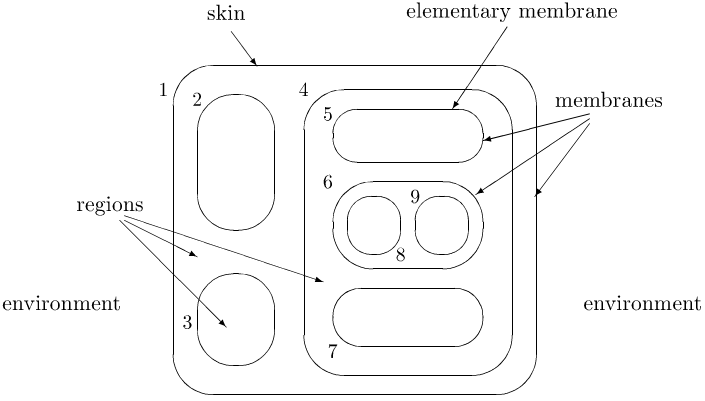
\includegraphics[width=0.7\textwidth]{membrane_structure.png}
      \hfill
      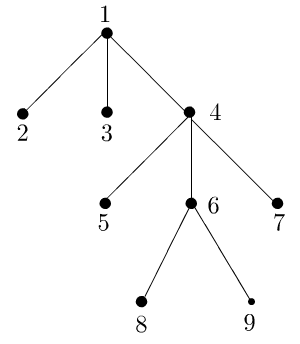
\includegraphics[width=0.3\textwidth]{membrane_tree.png}

    \end{frame}
    \note{}

    \begin{frame}[t]\frametitle{Contents of the membrane}
      \begin{itemize}
        \item multiset of objects
        \begin{itemize}
          \item $a\ |\ b\ |\ b$
        \end{itemize}
        \item rewriting rules
        \begin{itemize}
          \item $a\ |\ b\ |\ b\rightarrow a\ |\ a_{out}\ |\ b_{in_{6}}$
          \item $b \rightarrow a\ |\ \delta$
        \end{itemize}
      \end{itemize}
    \end{frame}
    \note{}

    \begin{frame}[t]\frametitle{P system}

      We define a P system as $\Pi = (V, \mu, w_1, w_2,\dots , w_m, R_1, R_2, \dots , R_m)$, where:
      \begin{itemize}
        \item $V$ is an alphabet of objects
        \item $\mu$ is a membrane structure
        \item $w_1, w_2, \dots w_m$ are initial multisets of objects in membranes $1\dots m$, $w_i\subseteq \mathbb{N}^V$
        \item $R_1, R_2, \dots , R_m$ are sets of rewriting rules in membranes $1\dots m$, where $$R_i\subseteq(\mathbb{N}^V\setminus 0^V)\times\mathbb{N}^{V\times(\{here,out\}\cup\{in_1,\dots in_m\})}$$.
      \end{itemize}

    \end{frame}
    \note{}

    \begin{frame}[t]\frametitle{Configuration and computational step}
      \begin{itemize}
        \item configuration = membrane structure + contents
        \item computational step: maximal parallelism
      \end{itemize}
      \tikzstyle{mybox} = [draw=black,very thick, rectangle, rounded corners, inner sep=10pt]
      \begin{tikzpicture}
        \onslide<2->{
          \node [mybox] (box){%
            \begin{minipage}{0.50\textwidth}
              \vspace{0pt}
              \begin{align}
                \tag{$r_1$}a\ |\ b\ |\ b&\rightarrow c\\
                \tag{$r_2$}b &\rightarrow c\ |\ c
              \end{align}
              $a\ |\ a\ |\ b\ |\ b$
            \end{minipage}
          };
        }
        \onslide<3->{
          \node [mybox,below=3cm of box.west,anchor=west] (box2) {$a\ |\ c$};
          \path[-triangle 45] (box) edge [left] node {$r_1$} (box2);
        }
        \onslide<4->{
          \node [mybox,below=3cm of box.east,anchor=east] (box3){$a\ |\ a\ |\ c\ |\ c\ |\ c\ |\ c$};
          \path[-triangle 45] (box) edge [right] node {$2*r_2$} (box3);
        }
      \end{tikzpicture}
    \end{frame}
    \note{}

    \begin{frame}[t]\frametitle{Language}
      \begin{itemize}
        \item result of the computation is a multiset of objects, which:
        \begin{itemize}
          \item have passed the outer membrane
          \item is present in a specific membrane at the end
        \end{itemize}
        \onslide<2->{\item generating vs. accepting mode}
        \onslide<3->{\item Parikh mapping: PsRE}
      \end{itemize}
    \end{frame}
    \note{}
    \newpage
    \note{}

  % subsection p_systems (end)

  \subsection{Variants} % (fold)
  \label{sub:variants}

    \begin{frame}[t]\frametitle{Variants of rules}
      \begin{itemize}
        \item context (PsRE)
        \onslide<2->{\item cooperative (PsRE) \cite{Paun98}}
        \onslide<3->{\item catalytic
          \begin{itemize}
            \item with 2 catalysts (PsRE) \cite{Freund2005TwoCatalysts}
            \item with 1 catalyst (open problem)
            \item with 1 catalyst and inhibitors (PsRE) \cite{Ionescu:jucs_10_5:on_p_systems_with}}
        \end{itemize}
        \onslide<4->{\item context-free (PsCF) \cite{Sburlan05dragos}}
        \onslide<5->{\item context-free with inhibitors (PsET0L) \cite{Ionescu:jucs_10_5:on_p_systems_with}}
      \end{itemize}
    \end{frame}
    \note{}
    \newpage
    \note{}

    \begin{frame}[t]\frametitle{Variants of computational step}
      \begin{itemize}
        \item maximal parallelism (PsRE)
        \onslide<2->{\item sequential (equals to VASS, \cite{Dang:2005:Sequential})}
        \onslide<3->{\item asynchronous ($\sim$ sequential in most cases) \cite{Freund:2004:APS:2144633.2144637}}
        \onslide<4->{\item minimal parallelism (PsRE) \cite{Ciobanu:2007:MinimalParallelism}}
        % \item n-paralelizmus, max-n-paralelizmus, \dots
      \end{itemize}
    \end{frame}
    \note{}

    \begin{frame}[t]\frametitle{Extensions of sequential P systems}
      \begin{itemize}
        \item priorities \cite{Dang:2005:Sequential}
        \item unbounded membrane creation \cite{Dang:2005:Sequential}
        \onslide<2->{\item {\bf inhibitors \cite[submitted]{Kovac14}}}
        \onslide<3->{\item further study (rules with emptyness detection, \dots)}
      \end{itemize}
    \end{frame}
    \note{}

  % subsection variants (end)

% section overview_of_p_systems (end)

\section{Sequential P systems with inhibitors} % (fold)
\label{sec:sequential_p_systems_with_inhibitors}

  \subsection{Accepting case} % (fold)
  \label{sub:accepting_case}
  
    \begin{frame}[t]\frametitle{Register machine}
      Minsky register machine is $M=(n,P,i,h)$, where:
      \begin{itemize}
        \item $n$ is the number of registers
        \item $P$ is a set of labeled instructions of type:
          \begin{itemize}
            \item $(add(r),k,l)$
            \item $(sub(r),k,l)$
            \item $halt$
          \end{itemize}
        \item $i$ is the initial instruction
        \item $h$ is the final instruction
      \end{itemize}
    \end{frame}
    \note{}

    \begin{frame}[t]\frametitle{Simulation of register machine}
      \begin{itemize}
        \item Contents of register $j$ is represented by the multiplicity of the object $a_j$
        \item For an instruction $(add(r),k,l)$ there is a rule $e\rightarrow a_j|f$
        \item For an instruction $(sub(r),k,l)$ there are rules
          \begin{itemize}
            \item $e|a_j\rightarrow f$
            \item $e\rightarrow z|_\not{a_j}$
          \end{itemize}
        \item Halting rules
          \begin{itemize}
            \item $h|a_j\rightarrow h|\#$ for all $a\leq j\leq n$
            \item $\#\rightarrow\#$
          \end{itemize}
      \end{itemize}
    \end{frame}
    \note{}

  % subsection accepting_case (end)

  \subsection{Generating case} % (fold)
  \label{sub:generating_case}

    \begin{frame}[t]\frametitle{Overview of the simulation for the generating case}
      \begin{itemize}
        \item Simulation of a maximal parallel step
        \item Phases of membranes: $RUN$ and $SYNCHRONIZE$, represented by objects
      \end{itemize}
    \end{frame}
    \note{}

    \begin{frame}[t]\frametitle{Major difficulties}
      \begin{itemize}
        \item Preventing the rule application on already rewritten objects in the same maximal parallel step
          \onslide<2->{\begin{itemize}
            \item replace objects on the right side $a$ with $a^{\prime}$ 
            \item add $RESTORE$ phase
          \end{itemize}}
        \onslide<3->{\item Sending objects via membranes
          \onslide<4->{\begin{itemize}
            \item add $SENDDOWN$ phase
          \end{itemize}}}
      \end{itemize}
    \end{frame}
    \note{}

    \definecolor{run}{rgb}{1,0.5,0}
    \definecolor{restore}{rgb}{0,0.5,0}
    \definecolor{synchronize}{rgb}{0,0,1}
    \definecolor{senddown}{rgb}{1,0,0}
    % Narrow texts in boxes
    \providecommand{\narrow}[1]{\scalebox{.8}[1.0]{#1}}

    \begin{frame}[t]\frametitle{Parent and child membrane phases}
      \begin{figure}
        \def\svgwidth{\textwidth}
        \input{possible_pairs_of_states_of_parent_and_child_membrane.pdf_tex}
        % 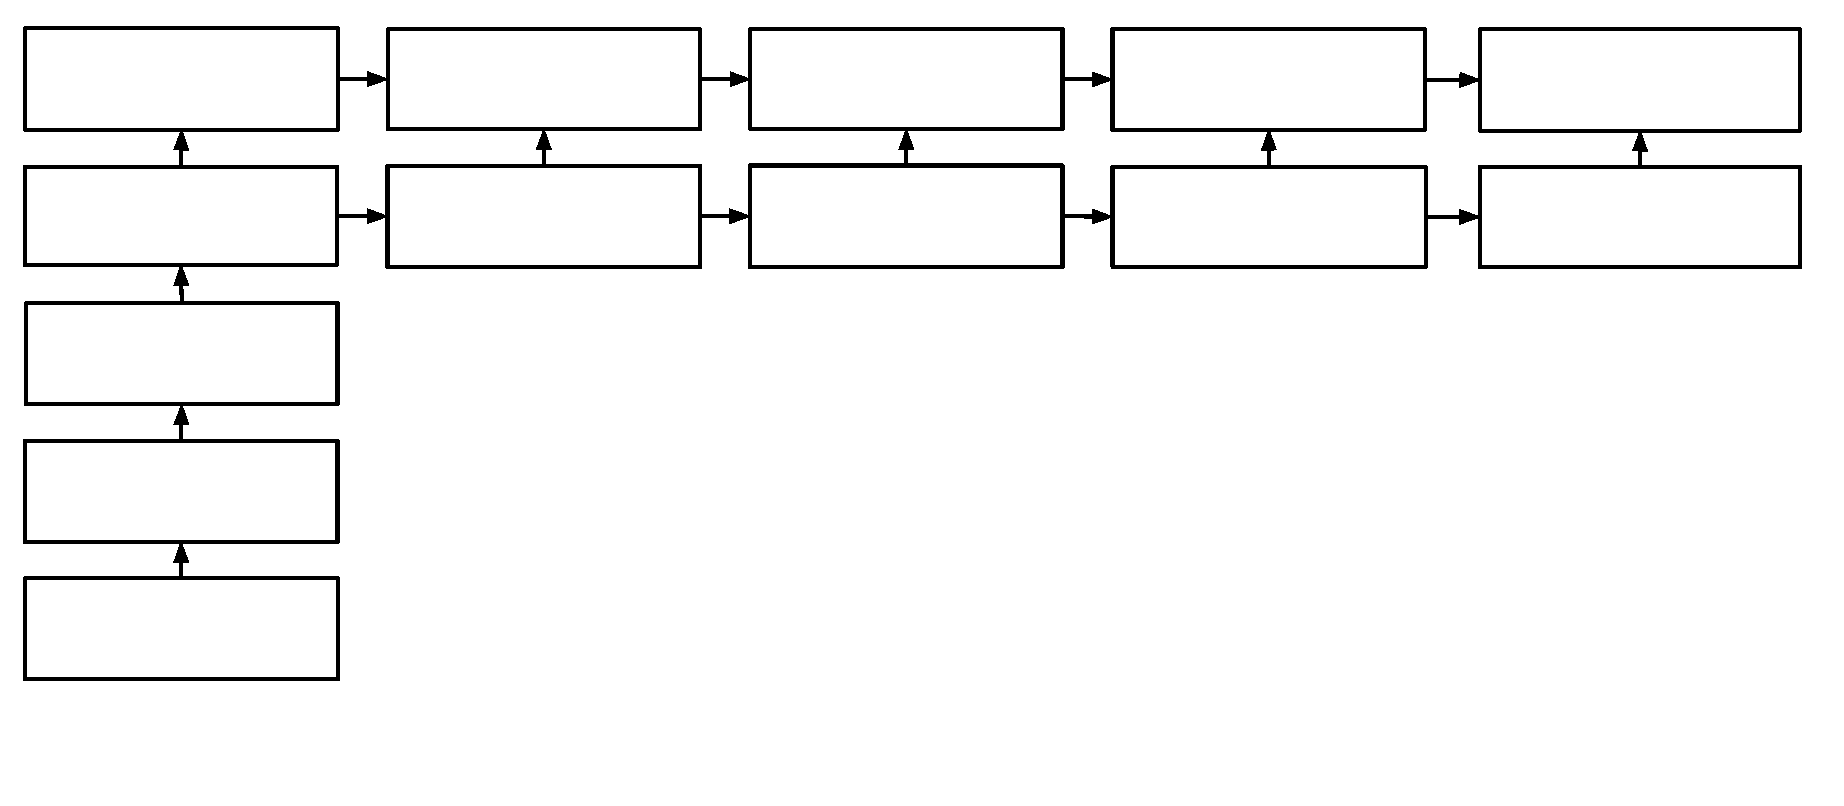
\includegraphics[width=\textwidth]{possible_pairs_of_states_of_parent_and_child_membrane}
        \caption{Possible pairs of states of parent and child membrane}
        \label{fig:possible_pairs_of_states_of_parent_and_child_membrane}
      \end{figure}
    \end{frame}
    \note{}

    \begin{frame}[t]\frametitle{Snapshot of all membrane states}
      \begin{figure}
        \def\svgwidth{\textwidth}
        \input{snapshot_of_all_membrane_states_while_simulating.pdf_tex}
        % 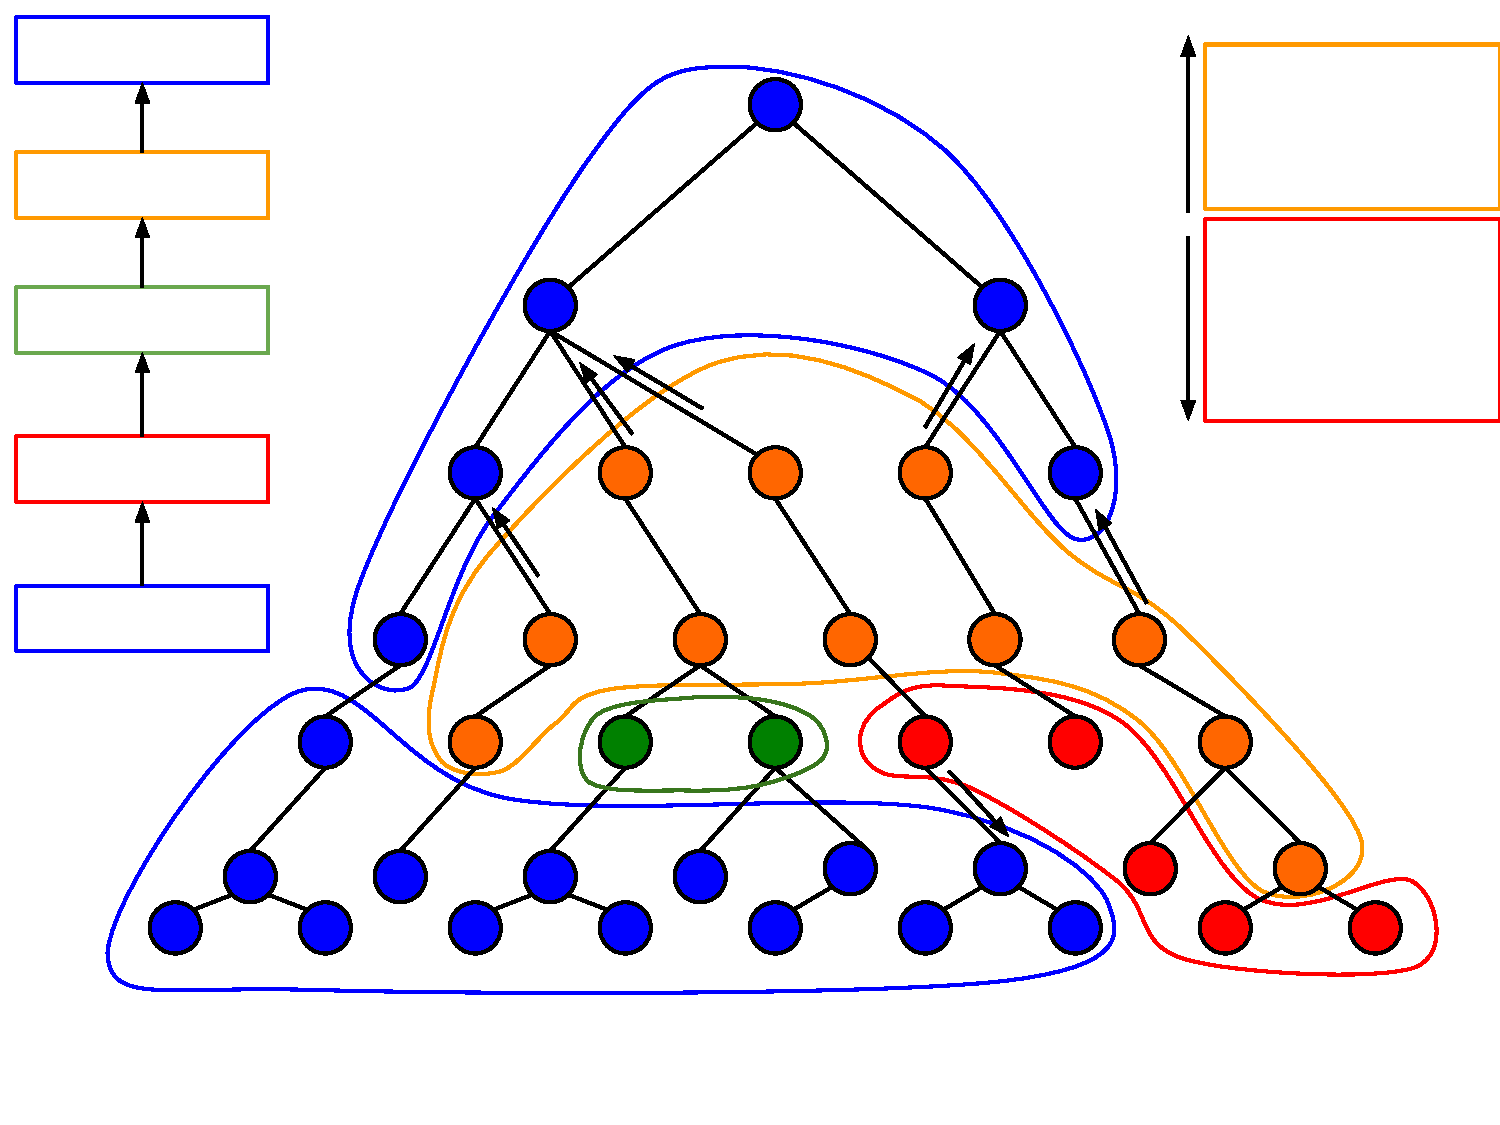
\includegraphics[width=\textwidth]{snapshot_of_all_membrane_states_while_simulating}
        \caption{Snapshot of all membrane states while simulating}
        \label{fig:snapshot_of_all_membrane_states_while_simulating}
      \end{figure}
    \end{frame}
    \note{}

  % subsection generating_case (end)

% section plany_na_dizertacnu_pracusequential_p_systems_with_inhibitors (end)

\begin{frame}[plain]
  \begin{center}
    Thanks for your attention
  \end{center}
\end{frame}

\newsavebox\mytempbib
\savebox\mytempbib{\parbox{\textwidth}{\bibliography{presentation}}}

\end{document}